\chapter{Revisão Bibliográfica}

\section{Trabalhos Correlatos}
\label{sec:related-work}

O problema de diarização de locutor é historicamente abordado de duas maneiras distintas.
A abordagem tradicional envolve a extração de vetores de características do áudio que se deseja diarizar, podendo ser estes \textit{I-Vectors} \cite{dehakFrontEndFactorAnalysis2011}, extraídos por meio de transformações matriciais aplicadas sobre o sinal, ou \textit{X-Vectors} \cite{snyderXVectorsRobustDNN2018}, obtidos através do uso de redes neurais profundas.
A partir de então, estes vetores podem ser clusterizados \cite{sellSpeakerDiarizationPlda2014} quando informações referentes ao número de locutores é conhecido, ou, mais recentemente, utilizados como entrada de uma rede neural LSTM \cite{wangSpeakerDiarizationLSTM2018}.

No entanto, a introdução das redes neurais convolucionais para reconhecimento de ações humanas em sinais de vídeos \cite{ji3DConvolutionalNeural2013, karpathyLargeScaleVideoClassification2014} implicou na concepção de uma nova abordagem.
Nesta, com o objetivo de melhorar a diarização de sinais heterogêneos, é utilizado um algoritmo de reconhecimento de ações também sobre o sinal de vídeo \cite{hersheyAudiovisualGraphicalModels2004}, que se supõe estar sincronizado ao áudio correspondente.
O reconhecimento de ações é, nesse caso, utilizado para identificar a fala do locutor e, quando combinado com os sinais de áudio, é capaz de produzir resultados melhores do que o estado da arte no processamento exclusivo de áudio \cite{ephratLookingListenCocktail2018}.

\section{Fundamentação Teórica}

\subsection{Redes Neurais Artificiais}
\label{sec:ann}

Redes Neurais Artificiais são um conjunto de algoritmos inspirados pelo funcionamento do cérebro humano, introduzidos pela primeira vez em 1943 quando Warren McCulloch e Walter Pitts modelaram o funcionamento de neurônios através de circuitos elétricos simples\cite{mccullochLogicalCalculusIdeas1943}. 
Esse modelo continuou evoluindo ao longo dos anos, culminando no desenvolvimento do \textit{Perceptron} por Rosenblatt em 1958 \cite{rosenblattPerceptronProbabilisticModel1958} (figura \ref{fig:perceptron}), um algoritmo de classificação binária semelhante a uma rede neural composta por um único neurônio.

No entanto, devido à falta de capacidade computacional e ao grande volume de dados necessários para o treinamento de redes neurais, estes algoritmos permaneceram apenas um conceito acadêmico durante vários anos.
Somente em 2006, Geoffrey Hinton proporia formalmente o conceito de rede neural profunda \cite{hintonFastLearningAlgorithm2006}, um tipo de rede neural composto por múltiplas camadas de neurônios totalmente conectadas.

\begin{figure}[ht]
    \centering
    \begin{tikzpicture}[]
    \node[coordinate] (input) [] {};
    \node[state, circle, align=center] (input1) at (input) [] {$x_2$};
    \node[state, circle, align=center] (input2) [above=of input1, yshift=-0.3cm] {$x_1$};
    \node[state, circle, align=center] (input3) [below=of input1, yshift=0.3cm] {$x_3$};
    \node[draw=none, fill=none] [below=of input3, yshift=-0.3cm] (inputs_label) {Entrada};

    \node[coordinate] (hidden1) [right=of input, xshift=1.5cm] {};
    \node[state, circle, align=center] (hidden11) at (hidden1) [] {};
        \draw [->, color=gray] (input1) -- (hidden11);
        \draw [->, color=gray] (input2) -- (hidden11);
        \draw [->, color=gray] (input3) -- (hidden11);
    \node[state, circle, align=center] (hidden12) [above=of hidden11, yshift=-0.7cm] {};
        \draw [->, color=gray] (input1) -- (hidden12);
        \draw [->, color=gray] (input2) -- (hidden12);
        \draw [->, color=gray] (input3) -- (hidden12);
    \node[state, circle, align=center] (hidden13) [above=of hidden12, yshift=-0.7cm] {};
        \draw [->, color=gray] (input1) -- (hidden13);
        \draw [->, color=gray] (input2) -- (hidden13);
        \draw [->, color=gray] (input3) -- (hidden13);
    \node[state, circle, align=center] (hidden14) [below=of hidden11, yshift=0.7cm] {};
        \draw [->, color=gray] (input1) -- (hidden14);
        \draw [->, color=gray] (input2) -- (hidden14);
        \draw [->, color=gray] (input3) -- (hidden14);
    \node[state, circle, align=center] (hidden15) [below=of hidden14, yshift=0.7cm] {};
        \draw [->, color=gray] (input1) -- (hidden15);
        \draw [->, color=gray] (input2) -- (hidden15);
        \draw [->, color=gray] (input3) -- (hidden15);

    \node[coordinate] (hidden2) [right=of hidden1, xshift=1.5cm] {};
    \node[state, circle, align=center] (hidden21) [above=of hidden2, yshift=-0.7cm] {};
        \draw [->, color=gray] (hidden11) -- (hidden21);
        \draw [->, color=gray] (hidden12) -- (hidden21);
        \draw [->, color=gray] (hidden13) -- (hidden21);
        \draw [->, color=gray] (hidden14) -- (hidden21);
        \draw [->, color=gray] (hidden15) -- (hidden21);
    \node[state, circle, align=center] (hidden22) [above=of hidden21, yshift=-0.7cm] {};
        \draw [->, color=gray] (hidden11) -- (hidden22);
        \draw [->, color=gray] (hidden12) -- (hidden22);
        \draw [->, color=gray] (hidden13) -- (hidden22);
        \draw [->, color=gray] (hidden14) -- (hidden22);
        \draw [->, color=gray] (hidden15) -- (hidden22);
    \node[state, circle, align=center] (hidden23) [below=of hidden2, yshift=0.7cm] {};
        \draw [->, color=gray] (hidden11) -- (hidden23);
        \draw [->, color=gray] (hidden12) -- (hidden23);
        \draw [->, color=gray] (hidden13) -- (hidden23);
        \draw [->, color=gray] (hidden14) -- (hidden23);
        \draw [->, color=gray] (hidden15) -- (hidden23);
    \node[state, circle, align=center] (hidden24) [below=of hidden23, yshift=0.7cm] {};
        \draw [->, color=gray] (hidden11) -- (hidden24);
        \draw [->, color=gray] (hidden12) -- (hidden24);
        \draw [->, color=gray] (hidden13) -- (hidden24);
        \draw [->, color=gray] (hidden14) -- (hidden24);
        \draw [->, color=gray] (hidden15) -- (hidden24);
    \node[draw=none, fill=none] [right=of inputs_label, xshift=0.25cm] (hidden_label) {Camadas Ocultas};

    \node[coordinate] (output) [right=of hidden2, xshift=1.5cm] {};
    \node[state, circle, align=center] (output1) [above=of output, yshift=-0.75cm] {$y_1$};
        \draw [->, color=gray] (hidden21) -- (output1);
        \draw [->, color=gray] (hidden22) -- (output1);
        \draw [->, color=gray] (hidden23) -- (output1);
        \draw [->, color=gray] (hidden24) -- (output1);
    \node[state, circle, align=center] (output2) [below=of output, yshift=0.75cm] {$y_2$};
        \draw [->, color=gray] (hidden21) -- (output2);
        \draw [->, color=gray] (hidden22) -- (output2);
        \draw [->, color=gray] (hidden23) -- (output2);
        \draw [->, color=gray] (hidden24) -- (output2);
    \node[draw=none, fill=none] [right=of hidden_label, xshift=0.25cm] (output_label) {Saída};

\end{tikzpicture}
    \caption{Ilustração de uma rede neural profunda com 3 camadas.}
    \label{fig:dnn}
\end{figure}

Recentemente, com o desenvolvimento de algoritmos para o treinamento de redes neurais em GPU (do Inglês \textit{Graphics Processing Unit}), que possibilitaram o treinamento mais rápido e eficiente de redes neurais de múltiplas camadas, assim como o crescente volume de dados disponível para treinamento, o tópico de redes neurais vem rapidamente ganhando popularidade.
Algoritmos desse tipo já são utilizados em diversas áreas da ciência, incluindo aplicações em medicina \cite{hannunCardiologistLevelArrhythmiaDetection2019,phamPredictingHealthcareTrajectories2017,houDeepSFDeepConvolutional2018}, previsão do tempo \cite{akramSequenceSequenceWeather2016}, veículos autônomos \cite{bojarskiEndEndLearning2016,peddagollaLaneDetectionAutonomous}, entre outras \cite{abiodunStateoftheartArtificialNeural2018}.

Tratam-se de algoritmos próprios para problemas que envolvem o reconhecimento de padrões, e a capacidade de treina-los a partir de dados existentes os torna eficazes para aplicação em tópicos nos quais as relações entre os dados de entrada não sejam totalmente conhecidas.

\subsubsection{Neurônios Artificiais}

Biologicamente, quando o potencial elétrico na base do axônio de um neurônio chega a um valor pré-determinado, por meio do acúmulo de sinais de entrada recebidos pelos dendritos, um pulso elétrico é gerado e propagado até as sinapses, terminais nos quais o neurônio conecta com os demais.
Trata-se de um sinal binário; o neurônio pode ou não estar ativado a cada instante. No entanto, a frequência relativa das ativações pode conter informação \cite{behnkeHierarchicalNeuralNetworks2003}.

\begin{figure}[H]
    \centering
    \includesvg[width=0.7\textwidth]{neurono-ido.svg}
    \caption{A estrutura de um neurônio biológico. Imagem adaptada de \cite{dhp1080IdoSkemoPri2016}.}
    \label{fig:bio_neuron}
\end{figure}

Funções de Ativação, também conhecidas como funções de propagação ou neurônios artificiais quando aplicadas no contexto de redes neurais, buscam modelar de forma simplificada esses aspectos biológicos.
Elas recebem como entrada os valores resultantes das camadas anteriores, ponderados por pesos específicos a cada conexão, e, quando estes valores atingem um limiar de excitação pré-determinado, os transformam em uma única saída.

\begin{figure}[H]
    \centering
    \begin{tikzpicture}
    \node[state, circle, align=center] (activation) [] {$\phi(x)$};
    
    \node[state, circle, align=center] (sum) [left=of activation] {$\sum$};
        \draw [->] (sum) -- (activation);
        
    \node[state, circle, align=center] (input1) [above left=of sum, yshift=-1cm, xshift=-1cm] {$x_2$};
        \draw [->] (input1) -- node [midway, above] {$w_2$} (sum);
        
    \node[state, circle, align=center] (input0) [above=of input1, yshift=-0.5cm] {$x_1$};
        \draw [->] (input0) -- node [midway, above] {$w_1$} (sum);
        
    \node[state, circle, align=center] (input2) [below left=of sum, yshift=1cm, xshift=-1cm] {$x_3$};
        \draw [->] (input2) -- node [midway, above] {$w_3$} (sum);
        
    \node[state, circle, align=center] (input3) [below=of input2, yshift=-0.5cm] {$x_n$};
        \path (input2) -- (input3) node [font=\Huge, midway, sloped] {$\dots$};
        \draw [->] (input3) -- node [midway, above=0.5em] {$w_n$} (sum);
        
    \node[draw=none, fill=none] [right=of activation] (output) {Saída};
        \draw [->] (activation) -- (output);
        
    \node[draw=none, fill=none] [below=of input3, yshift=0.7cm] (inputs) {Entradas};

\end{tikzpicture}
    \caption{O \textit{Perceptron}, uma rede neural com um único neurônio.}
    \label{fig:perceptron}
\end{figure}

Geralmente, a função de ativação é constante e independente do processo de treinamento da rede neural; o ajuste é feito sobre os pesos das conexões, através algoritmo de retropropagação \cite{dreyfusArtificialNeuralNetworks1990}.
O algoritmo é capaz de, a partir do resultado de uma camada, calcular o efeito de cada peso sobre o gradiente da função.
Assim, ele possibilita a utilização de algoritmos tradicionais de otimização para encontrar os pesos locais de cada conexão, mesmo em redes com múltiplas camadas de centenas de neurônios, em função do efeito global destes.

Comumente, são utilizadas como função de ativação as funções ReLU (\textit{Rectified Linear Unit}), tangente hiperbólica, sigmoide, e Heaviside, em função do intervalo de saída e comportamento desejado.

\begin{equation}\label{eq:relu}
    \phi(x) = \left\{
        \begin{array}{ll}
            0, & x \le 0\\
            x, & x > 0
        \end{array}
    \right.
\end{equation}

A função ReLU (equação \ref{eq:relu}), utilizada neste trabalho, tem comportamento tal que sua ativação ocorre sempre que $x>0$, com o valor resultante sendo o próprio valor de $x$. 
Essa função é ideal para aplicações em redes neurais profundas pois o gradiente é preservado após cada camada da rede, o que não ocorre com as funções sigmoide e tangente hiperbólica.
Nessas, o gradiente tende a valores infinitesimalmente pequenos após camadas sucessivas, dificultando o uso do algoritmo de retropropagação.
Além disso, o treinamento de redes neurais profundas que utilizam a função ReLU é mais rápido do que o das outras funções de ativação, devido à sua simplicidade \cite{krizhevskyImageNetClassificationDeep2017}.

\subsubsection{Redes Neurais Convolucionais}
\label{sec:convnet}

Redes Neurais Convolucionais são redes neurais compostas por uma ou mais camadas de convolução.
São ideais para o tratamento de dados matriciais, como por exemplo imagens, que constituem em uma matriz bi-dimensional de pixels, ou vídeos, matrizes tridimensionais de imagens.
Essas redes são capazes de identificar relações entre os elementos adjacentes de uma matriz, e, através da técnica de Max Pooling, focar somente nos pontos mais relevantes, mesmo em conjuntos de dados muito grandes.

\paragraph{Convolução e Filtros}
\label{sec:convolution}

A convolução é uma técnica matemática que consiste na aplicação de uma matriz, denominada matriz de convolução ou \textit{filtro} quando utilizada no contexto de processamento de imagens, sobre cada elemento de uma outra matriz.
Esse processo produz uma nova matriz na qual o valor de cada elemento corresponde ao seu valor e o valor de seus vizinhos, ponderados pelos valores da matriz de convolução, denominados \kernel\ da convolução.

Para dados bi-dimensionais, a operação de convolução pode ser descrita da seguinte forma:

\begin{equation}
    g(x,y) = \omega * f(x,y) = \sum\limits_{s=-a}^a\sum\limits_{t=-b}^b\omega(s,t)f(x-s, y-t)
\end{equation}

Essa técnica é frequentemente utilizada em áreas que trabalham com imagens, como na área de veículos autônomos, onde é capaz de identificar as faixas pintadas sobre o asfalto \cite{peddagollaLaneDetectionAutonomous}, assim como outros veículos e pedestres na rua.
Com a aplicação dessa, é possível remover características da imagem de entrada irrelevantes para o problema que se deseja resolver, como mostra a figura \ref{fig:conv}, diminuindo a complexidade do problema a cada camada.

\begin{figure}[ht]
    \centering
    \begin{tikzpicture}
    \node[inner sep=0pt] (pre_conv)
        {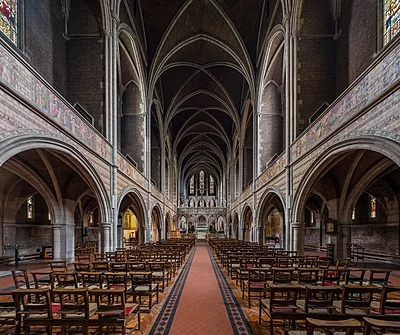
\includegraphics[width=0.3\textwidth]{photo_conv_1.png}};
    \node[state, rectangle, align=center] (kernel) [right=of pre_conv] 
        {
            $
                \begin{bmatrix}
                    0 & -1 & 1 \\
                    0 & -1 & 1 \\
                    0 & -1 & 1
                \end{bmatrix}
            $\\
            \textit{Kernel}
        };
        \draw [->] (pre_conv) -- (kernel);
    \node[inner sep=0pt] (post_conv) [right=of kernel]
        {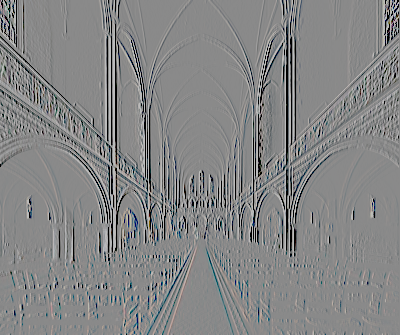
\includegraphics[width=0.3\textwidth]{photo_conv_2.png}};
        \draw [->] (kernel) -- (post_conv);
\end{tikzpicture}
    \caption{O resultado da aplicação de um \kernel\ simples para detecção de bordas verticais a uma foto. 
    O \kernel\ é aplicado a cada pixel da imagem, substituindo o valor deste pela soma de sua vizinhança ponderada pelos valores da matriz. 
    Foto original obtida de \cite{diliffEnglishLookingEast2015}.}
    \label{fig:conv}
\end{figure}

No contexto de redes neurais convolucionais, isso consiste em neurônios que realizam uma operação de convolução sobre os dados de entrada.
O \kernel\ da matriz de convolução é treinado de forma a identificar os aspectos da entrada mais relevantes para o problema, através do algoritmo de retropropagação.

\paragraph{Pooling}
\label{sec:pooling}

Um outro tipo de camada tradicional nas redes neurais convolucionais é a camada de \textit{pooling}, ou ``agrupamento''.
Esse tipo de camada tem como função reduzir o número e complexidade dos dados de entrada e promover uma melhor generalização dos dados espaciais.
Isso é necessários pois as camadas convolucionais tendem a manter a localização espacial das características detectadas na matriz de entrada, informação que na maioria dos casos não é relevante para o problema que se deseja resolver.

A operação consiste em subdividir a matriz de entrada em conjuntos de valores e, segundo um critério especificado, escolher entre estes um único valor resultante.

\begin{figure}[ht]
    \centering
    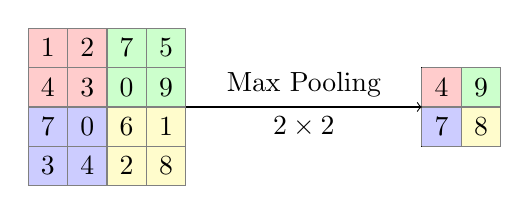
\begin{tikzpicture}
    \filldraw[fill=red!20!white] (-1, 1) rectangle (0, 0);
    \filldraw[fill=green!20!white] (0, 1) rectangle (1, 0);
    \filldraw[fill=blue!20!white] (-1, -1) rectangle (0, 0);
    \filldraw[fill=yellow!20!white] (0, 0) rectangle (1, -1);
    \draw[step=0.5cm, color=gray] (-1, -1) grid (1, 1);
    \node[coordinate] (pre_pool) at (1, 0) {};
    \node at (-0.75, +0.75) {1};
    \node at (-0.25, +0.75) {2};
    \node at (+0.25, +0.75) {7};
    \node at (+0.75, +0.75) {5};
    \node at (-0.75, +0.25) {4};
    \node at (-0.25, +0.25) {3};
    \node at (+0.25, +0.25) {0};
    \node at (+0.75, +0.25) {9};
    \node at (-0.75, -0.25) {7};
    \node at (-0.25, -0.25) {0};
    \node at (+0.25, -0.25) {6};
    \node at (+0.75, -0.25) {1};
    \node at (-0.75, -0.75) {3};
    \node at (-0.25, -0.75) {4};
    \node at (+0.25, -0.75) {2};
    \node at (+0.75, -0.75) {8};

    \filldraw[fill=red!20!white] (4, 0.5) rectangle (4.5, 0);
    \filldraw[fill=green!20!white] (4.5, 0.5) rectangle (5, 0);
    \filldraw[fill=blue!20!white] (4, 0) rectangle (4.5, -0.5);
    \filldraw[fill=yellow!20!white] (4.5, 0) rectangle (5, -0.5);
    \draw[step=0.5cm, color=gray] (4-0.001, -0.5) grid (5, 0.5);
    \node[coordinate] (post_pool) at (4, 0) {};
    \node at (4.25, +0.25) {4};
    \node at (4.25, -0.25) {7};
    \node at (4.75, +0.25) {9};
    \node at (4.75, -0.25) {8};

    \draw[->] (pre_pool) -- (post_pool);
    \path [] (pre_pool) -- node [midway, above] {Max Pooling} node [midway, below] {$2\times2$} (post_pool);
\end{tikzpicture}
    \caption{O resultado da operação de \textit{Max Pooling} com dimensão $2\times2$ sobre uma matriz de entrada.}
    \label{fig:maxpool}
\end{figure}

No contexto de redes neurais convolucionais, no entanto, dado que os valores resultantes da camada convolucional teriam sido filtrados por uma função de ativação não-linear, como a ReLU (equação \ref{eq:relu}), temos que os valores obtidos correspondem à intensidade da ativação dos neurônios.
Assim, devido ao fato de que valores maiores devem corresponder a características de maior importância na matriz de entrada, temos dois critérios mais usados para a operação:

\begin{description}
    \itemsep0em 
    \item \textit{\textbf{Max Pooling}}: Para cada grupo, calcula o valor máximo (figura \ref{fig:maxpool}).
    \item \textit{\textbf{Average Pooling}}: Para cada grupo, calcula a média dos valores.
\end{description}

A escolha entre esses critérios é feita em função do propósito da camada anterior; se esta for, por exemplo, um detector de bordas em imagens, temos que a técnica de \textit{Max Pooling} será preferível, visto que as bordas serão sempre o maior valor do grupo, enquanto os demais elementos terão valor zero.
Já no caso de se tratar de um reconhecedor de variação temporal, a técnica de \textit{Average Pooling} pode ser preferível, já que será capaz de manter informações sobre o valor médio dos elementos no instante que está sendo comprimido.

\subsection{Histograma de Gradientes Orientados}
\label{sec:facialrecog}

Histograma de Gradientes Orientados, ou HOG, do inglês \textit{Histogram of Oriented Gradients}, é uma técnica de visão computacional utilizada para detecção de objetos em imagens.

\begin{figure}[ht]
    \centering
    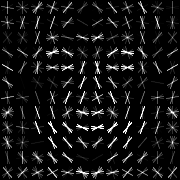
\includegraphics[width=0.30\textwidth]{face_fhog_filters.png}
    \caption{HOG para identificação facial frontal. Imagem retirada de \cite{kingDlib18Released}.}
    \label{fig:dlib_hog}
\end{figure}

\subsection{Detecção de Marcadores Faciais}
\label{sec:faciallm}